\section{Regelkreis aus LZI}
\subsection{Gegenkopplung}
\script{109} Wenn bei einem Regelkreis $e = -y$ gilt, ist dieser Grenzstabil. Dafür müssen bei einem \underline{offenen} Regelkreis die Frequenz $\omega$, und Totzeit $T_t$ korrekt gewählt werden.

Bei einem \underline{geschlossenen} Regelkreis, müssen Parameter korrekt eingestellt sein. Dabei ist die Frequenz $\omega$ gegeben und entspricht der Eigenfrequenz.
\begin{center}
	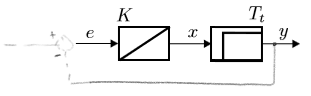
\includegraphics[width=0.7\columnwidth]{Images/grenzstabil}
\end{center}


\subsection{Kaskadierung}
Serien-Schaltungen werden multipliziert (Matlab: \textit{series(s1, s2)}). Parallel-Schaltung werden addiert/subtrahiert (Matlab: \textit{parallel(s1, s2)}). Rückkopplung nur mit (Matlab: \textit{feedback(s1, s2,+1)})
\begin{center}
	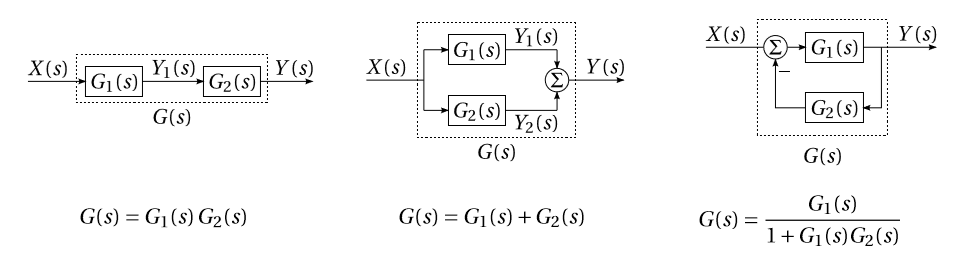
\includegraphics[width=\columnwidth]{Images/systeme}
\end{center}